\documentclass[a4paper,11pt]{report}
\usepackage{pywps}
\usepackage{layout}
\usepackage{lscape}
\usepackage[utf8]{inputenc}
\usepackage[dvips]{graphicx}
\usepackage{url}
\usepackage[colorlinks=true]{hyperref}
\usepackage[table,dvipsnames]{xcolor}[2004/07/04]

\author{PyWPS Development team\thanks{\url{http://wald.intevation.org/projects/pywps/http://wald.intevation.org/projects/pywps/}}}

\title{Implementation of OGC WPS standard: PyWPS}

\date{\today\\{}\vspace{2cm}
\includegraphics[width=5cm]{pic/pywps.png}}

\pagestyle{plain}

\begin{document}
\maketitle{}

\bigskip
\begin{quote}
    Copyright \copyright  2006-2009 PyWPS Development Team
    Permission is granted to copy, distribute and/or modify this document
    under the terms of the GNU Free Documentation License, Version 1.2
    or any later version published by the Free Software Foundation;
    with no Invariant Sections, no Front-Cover Texts, and no Back-Cover Texts.
    A copy of the license is included in the section entitled "GNU
    Free Documentation License".
\end{quote}
\bigskip


In this file, you can found the description of installation and
configuration of PyWPS script. At the and, you can learn, how to add
your own process. This document describes most recent
version of PyWPS (\version), available in subversion repository.

PyWPS project has been started on April 2006 with support of DBU --
Deutsche Bundesstiftung Umwelt\footnote{\url{http://dbu.de}} and with help of
GDF-Hannover\footnote{\url{http://gdf-hannover.de}} and Help Service Remote
Sensing\footnote{\url{http://www.bnhelp.cz}} companies. Initial author is Jachym
Cepicky\footnote{\url{http://les-ejk.cz}}.
    
\chapter{Changes}
Changes of this document
\begin{description}
    \item [2008-10-06] Updated according to new PyWPS version (3.0.0) \jachym
\end{description}

\tableofcontents

\newpage

%---------------------------------------------------------------------
\chapter{Introduction}
PyWPS (Python Web Processing Service) is implementation of Web
Processing Service 1.0.x standard from Open Geospatial
Consortium\footnote{\url{http://www.opengeospatial.org/standards/requests/28}}.

It has been started on Mai 2006 as project supported by DBU. It offers
environment for programming own process (geofunctions or models) which can
be accessed via HTTP protocol from various clients. The main advantage of PyWPS is, that it has
been written with native support for GRASS
GIS\footnote{\url{http://grass.itc.it}}. Access GRASS modules via web
interface should be as easy as possible.
However, not only GRASS GIS is supported. Usage of other programs, like
R package or GDAL or PROJ tools is possible as well.

PyWPS is written in Python programming language, your processes must use
this language too. However, this does not mean, that you have to write all
your processes using Python. You can write single scripts/programs in any
programming language you are used to. In Python, you have to setup only
small wrapper file, which will call your custom processes and provide the
response back to the client.

PyWPS Homepage can be found at \url{http://pywps.wald.intevation.org}.
PyWPS Wiki is hosted on \url{http://pywps.ominiverdi.org/wiki}.

\section{How it works}
PyWPS is a translator-proxy application between client (Web Browser, Desktop
GIS, command line tool, \dots) and working tool installed on the server.
PyWPS does not process the data by it self. As working tool, GRASS GIS, GDAL, PROJ, R
and other programs can be used.

\begin{figure}[ht]
\begin{center}
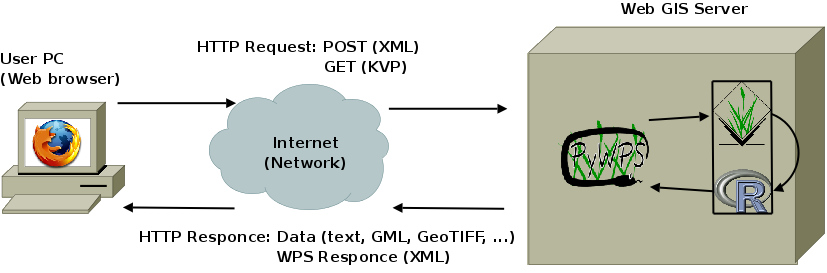
\includegraphics[width=1\textwidth]{pic/pywps-schema}
\caption{How does PyWPS work: GRASS GIS is in this case working tool}
\label{pic:pywps}
\end{center}
\end{figure}

%---------------------------------------------------------------------
\chapter{Installation}
\label{install}   
Required packages:
    
\begin{itemize}
    \item python 
    \item python-xml 
    \item python-htmltmpl 
\end{itemize}
    
Recommended packages:
    
\begin{itemize}
    \item Web Server (e.g. Apache) -- \url{http://httpd.apache.org} -  You
    will need an web server, to be able to execute processes from remote
    computers.

    \item GIS GRASS  -- \url{http://grass.itc.it} - Geographical Resources
    Analysis Support System (GRASS) is Open Source GIS, which provides more
    then 350 modules for raster and vector (2D, 3D) data analysis. PyWPS is
    written with native support for GRASS and it's functions.

    \item PROJ.4  -- \url{http://proj.maptools.org} - Cartographic
    Projections library used in various Open Source projects, such as
    GRASS, UMN MapServer, QGIS and others. It can be used e.g. for data
    transformation.

    \item GDAL/OGR  -- \url{http://gdal.org} - translator library for
    raster geospatial data formats, is used in various projects for
    importing, exporting and transformation between various raster and vector
    data formats.

    \item R  -- \url{http://www.r-project.org} - is a language and environment
    for statistical computing and graphics.

\end{itemize}
    
\section{Installation the quick 'n' dirty way}
For installing PyWPS to your server simply unpack the archive to the
directory, where CGI programs are allowed to run. You can also use current
repository version.

\begin{verbatim}
$ cd /usr/lib/cgi-bin/
$ tar xvzf /tmp/pywps-VERSION.tar.gz
$ pywps/wps.py
\end{verbatim}

\subsection{Post-installation steps}
You have to change the write access of \texttt{pywps/Templates} directory,
so the web server can compile the templates:
\begin{verbatim}
chmod 777 pywps/Templates/1_0_0
\end{verbatim}

The default location of the configuration file is
\texttt{pywps/etc/pywps.cfg}. The default location of the processes
directory is \texttt{pywps/processes}. NOTE: See
section~\ref{environment_variables} how to customize the location of
configuration files and processes directory.

\section{Installation the 'clean' way}
Unpack the package 
\begin{verbatim}
$ tar -xzf pywps-VERSION.tar.gz
\end{verbatim}
and run 
\begin{verbatim}
$ python setup.py install
\end{verbatim} 

The default location of the configuration file is
\texttt{/etc/pywps.cfg} on Unix or
\texttt{PYWPS\_INSTALLATION\_PATH/pywps/etc/pywps.cfg} on Windows. The default location of the processes
directory is on \texttt{PYWPS\_INSTALLATION\_PATH/pywps/processes/}. On
Unix, \texttt{PYWPS\_INSTALLATION\_PATH} is something similar to
\texttt{/usr/lib/python2.5/site-packages/}.
NOTE: See section~\ref{environment_variables} how to customize the location of
configuration file and processes directory.

\section{PyWPS Environment variables}
\label{environment_variables}
Several environment variables can be set (see section~\ref{wrapper_script}
for examples), to change the default PyWPS behaviour:
\begin{description}
    \item[\texttt{PYWPS\_CFG}] Location of the PyWPS configuration file.
    Default is \texttt{/etc/pywps.cfg} or
    \texttt{PYWPS\_INSTALLATION\_PATH/pywps/etc/pywps.cfg}.

    \item[\texttt{PYWPS\_PROCESSES}] Location of the processes directory
    (python-package). The directory contains \texttt{\_\_init\_\_.py}
    configuration script, as well as all processes.
\end{description}

\section{PyWPS as CGI}
\subsection{Symlink}
If you did not installed PyWPS to \texttt{cgi-bin} directory of your
server, you can create the symlink in \texttt{cgi-bin} to \texttt{wps.py}:
\begin{verbatim}
ln -s /usr/bin/wps.py /usr/lib/cgi-bin/wps.py
\end{verbatim}
In this case, options \texttt{+ExecCGI +FollowSymLinks} must be enabled for
\texttt{cgi-bin} directory in the web server configuration file. Example:
\begin{verbatim}
# /etc/apache2/sites-enabled/000-default
# ...
        ScriptAlias /cgi-bin/ /usr/lib/cgi-bin/
        <Directory "/usr/lib/cgi-bin">
                AllowOverride None
                Options +ExecCGI -MultiViews +FollowSymLinks
                Order allow,deny
                Allow from all
        </Directory>
# ...
\end{verbatim}

\subsection{Wrapper script}
\label{wrapper_script}
You can also write little wrapper script, which will setup environment
variables and run \texttt{wps.py} script. In this case, you can create
several WPS servers  (separate sets of processes) with only one PyWPS
installation. Example follows:
\begin{verbatim}
#!/usr/sh

# Author: jachym
# Purpose: PyWPS wrapper script
# Licence: GNU/GPL
# Version: To be used with PyWPS >= 3.0.0
# Installation: Put this script to /usr/lib/cgi-bin directory (or other
#               cgi-bin directory of your web server) and call it whatever
#               you like (e.g. "foowps"). Adjust the variables below and 
#               chmod +x this script.

export PYWPS_CFG=/usr/local/pywps/foo/pywps.cfg
export PYWPS_PROCESSES=/usr/local/pywps/foo/processes/

/usr/bin/wps.py
\end{verbatim}

%---------------------------------------------------------------------
\chapter{Configuration}
\label{configuration}
    
Before you start to tune your PyWPS installation, you should get your copy of
OpenGIS(R) Web Processing Service document (OGC  05-007r7) version
1.0.0\footnote{\url{http://www.opengeospatial.org/standards/wps}}.
    
\note{Note, that the configuration option are CASE SENSITIVE}
    
Pywps configuration takes place in \texttt{pywps.cfg} file located in
\texttt{/etc/pywps.cfg} or \texttt{pywps/etc/pywps.cfg}. Path to the
configuration file can be also set by the \texttt{PYWPS\_CFG} environment
variable (section \ref{environment_variables}), see
section~\ref{wrapper_script} for example usage.

Default configuration file is located in \texttt{pywps/default.cfg}, you
can always make a copy of this file and start the configuration from
scratch.
    
Several sections are in the file. 
\begin{itemize}
    \item Section \textbf{[wps]} contains general WPS settings, which are:
        \begin{itemize}
            \item encoding -- Language encoding (utf-8, iso-8859-2, windows-1250, \dots)
            \item title -- Server title 
            \item version -- WPS version (1.0.0)
            \item abstract -- Server abstract
            \item fees -- Possible fees
            \item constraints -- Possible constraints
            \item serveraddress -- WPS script address: \url{http://foo/bar/wps.py}
            \item keywords -- Comma-separated list of keywords
            \item lang -- Default language (eng)
        \end{itemize}
    \item Section \textbf{[provider]} contains informations about you
        \begin{itemize}
            \item providerName -- Name of your company
            \item individualName -- Your name
            \item positionName
            \item role 
            \item deliveryPoint -- Street
            \item city
            \item postalCode
            \item country
            \item electronicMailAddress -- foo@bar
            \item providerSite -- \url{http://foo.bar}
            \item phoneVoice
            \item phoneFacsimile
            \item administrativeArea
        \end{itemize}
    \item Section \textbf{[server]} contains server settings
        \begin{itemize}
            \item maxoperations -- Maximal number of parallel running
            processes. If set to 0, then there is no limit.
            \item maxinputparamlength -- Maximal length of string input
            parameter.
            \item maxfilesize -- Maximal input file size (raster or
            vector). The size can be determined as follows: 1GB, 5MB, 3kB,
            1000b.
            \item tempPath -- Directory for temporary files (mostly
            temporary GRASS locations).
            \item outputUrl -- Url where the outputs are stored.
            \item outputPath -- Path. where output files are stored.
            \item debug -- true/false
            \item processesPath -- path to your processes. Default is
            \texttt{pywps/processes}. 

            NOTE: You can set also \texttt{PYWPS\_PROCESSES} environment
            variable with same result (section~\ref{environment_variables}).
        \end{itemize}
    \item Section \textbf{[grass]} -- GRASS GIS settings
        \begin{itemize}
            \item path -- \$PATH variable, e.g. \texttt{/usr/lib/grass/bin}
            \item addonPath -- \$GRASS\_ADDONS variable
            \item version -- GRASS version
            \item gui -- Should be "text"
            \item gisbase -- Path to GRASS GIS\_BASE directory
            (\texttt{/usr/lib/grass})
            \item ldLibraryPath -- Path of GRASS Libs
            (\texttt{/usr/lib/grass/lib})
	    \item gisdbase -- Full path to location directory 
	    (\texttt{/home/foo/grassdata}) NOTE: You do not have to setup
            this variable in the configuration file globaly. You can use
            \texttt{grassLocation} attribute while calling the
            \texttt{\_\_init\_\_} method of Process class, while process
            initialization. See section~\ref{processes} for more details.
        \end{itemize}
\end{itemize}

File example follows:
\begin{verbatim}
[wps]
encoding=utf-8
title=PyWPS Server
version=1.0.0
abstract=See http://pywps.wald.intevation.org and http://www.opengeospatial.org/standards/wps
fees=None
constraints=none
serveraddress=http://localhost/cgi-bin/wps
keywords=GRASS,GIS,WPS
lang=eng

[provider]
providerName=Your Company Name
individualName=Your Name
positionName=Your Position
role=Your role
deliveryPoint=Street
city=City
postalCode=000 00
country=eu
electronicMailAddress=login@server.org
providerSite=http://foo.bar
phoneVoice=False
phoneFacsimile=False
administrativeArea=False

[server]
maxoperations=3
maxinputparamlength=1024
maxfilesize=3mb
tempPath=/tmp
processesPath=
outputUrl=http://localhost/wps/wpsoutputs
outputPath=/var/www/wps/wpsoutputs
debug=true

[grass]
path=/usr/lib/grass/bin/:/usr/lib/grass/scripts/
addonPath=
version=6.2.1
gui=text
gisbase=/usr/lib/grass/
ldLibraryPath=/usr/lib/grass/lib
gisdbase=/home/foo/datagrass
\end{verbatim}
    
\subsection{Testing after installation}
\label{testing}
For test, just run
\texttt{wps.py} in the terminal. The WPS options can be written as
parameter:
    
\begin{verbatim}
$ wps.py "service=wps&request=getcapabilities"

INIT DONE
LOADING PRECOMPILED
TEMPLATE: UPTODATE
PRECOMPILED: UPTODATE
Content-type: text/xml

<?xml version="1.0" encoding="utf-8"?>
<wps:Capabilities service="WPS" version="1.0.0" xml:lang="eng,ger"
    xmlns:xlink="http://www.w3.org/1999/xlink"
    xmlns:wps="http://www.opengis.net/wps/1.0.0"
    xmlns:ows="http://www.opengis.net/ows/1.1"
    xmlns:xsi="http://www.w3.org/2001/XMLSchema-instance
    xsi:schemaLocation="http://www.opengis.net/wps/1.0.0
    http://schemas.opengis.net/wps/1.0.0/wpsGetCapabilities_response.xsd"
    updateSequence="1">
	<ows:ServiceIdentification>
		<ows:Title>PyWPS Development Server</ows:Title>
    ...
</wps:Capabilities>
\end{verbatim}

If you got something like this, (Capabilities response), everything looks
fine.
     
If you got some other message, like e.g.:
     
\begin{verbatim}
Traceback (most recent call last):
  File "/usr/bin/wps.py", line 221, in <module>
    wps = WPS()
  File "/usr/bin/wps.py", line 140, in __init__
    self.performRequest()
  File "/usr/bin/wps.py", line 188, in performRequest
    from pywps.WPS.GetCapabilities import GetCapabilities
  File "/usr/lib/python2.5/site-packages/pywps/WPS/GetCapabilities.py", line 26, in <module>
    from Response import Response
  File "/usr/lib/python2.5/site-packages/pywps/WPS/Response.py", line 28, in <module>
    from htmltmpl import TemplateManager, TemplateProcessor
ImportError: No module named htmltmpl
\end{verbatim}

     
Than something is wrong with your Python installation or with the program.
This message means, that the python-htmltmpl package is not installed in
your system.
     
%---------------------------------------------------------------------
\chapter{Write your own processes}
\label{processes}
    
The default location for processes is \texttt{PYWPS\_INSTALLATION\_PATH/pywps/processes}. You can
create custom directory anywhere in your system and set
\texttt{\$PYTHON\_PROCESS} environmental variable (on how to do this for the web
server, refer to your Server documentation, see sections
\ref{wrapper_script} and \ref{environment_variables} for details).

Alternatively you can set the \texttt{processesPath} variable in the configuration file.
Following example will describe buffering process. Several example processes are 
distributed along with PyWPS source code (they are in the
\texttt{doc/examples/processes} directory) -- feel free to get inspired by
them.

\section{Process initialization and configuration}
\begin{enumerate}
\item Create file \texttt{foo.py} in \texttt{PYWPS\_PROCESSES} directory.
\item Add \texttt{foo} to \texttt{\_\_all\_\_} array in the \texttt{\_\_init\_\_.py}
file.
\end{enumerate}
    
Each process is stand-alone python script with one class \texttt{Process},
which has two methods: \texttt{\_\_init\_\_, execute}. It is possible also to add as 
many your functions/methods, as you wish.
    

\begin{verbatim}
  1 from pywps.Process.Process import WPSProcess                                
  2 class Process(WPSProcess):
  3     """Main process class"""
  4     def __init__(self):
  5         """Process initialization"""
  7         # init process
  8         WPSProcess.__init__(self,
  9             identifier = "foo", # must be same, as filename
 10             title="Buffer",
 11             version = "0.2",
 12             storeSupported = "true",
 13             statusSupported = "true",
 14             abstract="Create a buffer around an input vector file",
 15             grassLocation = True)
\end{verbatim}

We defined new process called \texttt{foo}. The process is allowed to
store it's output data on the server (\texttt{storeSupported}) and it is also possible to run it in
asynchronous mode (\texttt{statusSupported}). The process will run within
GRASS GIS environment (\texttt{grassLocation = True}) -- temporary location
will be created and deleted again, after the processes is done.


\paragraph{Mandatory parameters of the \texttt{\_\_init\_\_} method:}
\begin{itemize}
        identifier \textbf{String} process identifier
        title \textbf{String} process title
\end{itemize}

\paragraph{Optional parameters:}
\begin{itemize}
\item abstract \textbf{String} process description
                default: None
\item metadata List of additional metadata.  See
                    http://www.opengeospatial.org/standards/common, table 32 on page 65
                E.g. ["foo":"bar"]\\
                default: None
\item profile [URN]\\
                default: None
\item version \textbf{String} process version\\
                default: None
\item statusSupported \textbf{Boolean} this process can be run
        asynchronously\\
                default: True
\item storeSupported \textbf{Boolean} outputs from this process can be stored
                for later download\\
                default: True
\item grassLocation \textbf{String} or {Boolean} name of GRASS Location within
                "gisdbase" directory (from pywps.cfg configuration file).
                If set to True, temporary GRASS Location will be created
                and grass environment will be started. If None or False, no
                GRASS environment will be started.\\
                default: None
\end{itemize}

     
\subsection{Data Inputs}

Three types of data inputs are defined:
\begin{itemize}
    \item Literal Input -- Basic literal input -- single number or text
    value
    \item ComplexValue Input  -- Mostly vector file will be included in input XML
    request. It can be also only referenced (only URL will be send).
    \item BoundingBox Input -- Coordinates for lower-left and upper-right
    corner.
\end{itemize}


\subsubsection{ComplexInput}
Complex input can be raster or vector file, to be processed. 

\begin{verbatim}
 18         self.dataIn = self.addComplexInput(identifier="data",
 19                              title = "Input data")
 20 
\end{verbatim}

\paragraph{Mandatory parameters:}
\begin{itemize}
    \item identifier \textbf{String} input identifier
    \item title \textbf{String} input title
\end{itemize}

\paragraph{Optional parameters:}
\begin{itemize}
\item abstract \textbf{String} input description.
        default: None
\item metadata List of \textbf{Dict} {key:value} pairs.
        default: None
\item minOccurs \textbf{Integer} minimum number of occurrences.
        default: 1
\item maxOccurs \textbf{Integer} maximum number of occurrences.
        default: 1
\item formats List of \textbf{Dict} according to table 23 (page 25). E.g.
    \begin{verbatim}
            [
                {"mimeType": "image/tiff"},
                {
                    "mimeType": "text/xml",
                    "encoding": "utf-8",
                    "schema":"http://foo/bar"
                }
            ]
    \end{verbatim}
        default: [{"mimeType":"text/xml"}]
\item maxmegabites \textbf{Float} Maximum input file size. Can not be bigger, as
        defined in global configuration file.\\
        default: 5
\end{itemize}



\subsubsection{LiteralInput}

With literal input, you can obtain any type of character string.

\begin{verbatim}
 21         self.widthIn = self.addLiteralInput(identifier = "width",
 22                              title = "Width")
 23 
\end{verbatim}

\paragraph{Mandatory parameters:}
\begin{itemize}
\item identifier \textbf{String} input identifier
\item title \textbf{String} input title
\end{itemize}

\paragraph{Optional parameters:}
\begin{itemize}
\item abstract \textbf{String} input description. Default: None
            default: None\\
\item uoms List of \textbf{String} value units\\
            default: ()
\item minOccurs \textbf{Integer} minimum number of occurrences.\\
            default: 1
\item maxOccurs \textbf{Integer} maximum number of occurrences.
            default: 1\\
\item allowedValues  List of {String} or {List} list of allowed values,
            which can be used with this input. You can set interval
            using list with two items, like:

            (1,2,3,(5,9),10,"a",("d","g"))

            This will produce allowed values 1,2,3,10, "a" and
            any value between 5 and 9 or "d" and "g".

            If "*" is used, it means "any value"\\
            default: ("*")
\item type \textbf{types.TypeType} value type, e.g. Integer, String, etc. you
            can uses the "types" module of python.\\
            default: types.IntType
\item default \textbf{Any} default value.\\
            default: None
\item metadata List of \textbf{Dict} Additional metadata. E.g.  {"foo":"bar"}\\
            default: None
\end{itemize}

\subsubsection{BoundingBox Input}
The input is added to the process using \texttt{addBBoxInput}.

\paragraph{Mandatory parameters:}
\begin{itemize}
\item identifier \textbf{String} input identifier
\item title \textbf{String} input title
\end{itemize}

\paragraph{Optional parameters:}
\begin{itemize}
\item abstract \textbf{String} input description.\\
        default: None
\item metadata List of \textbf{Dict} {key:value} pairs.\\
        default: None
\item minOccurs \textbf{Integer} minimum number of occurrences.\\
        default: 1
\item maxOccurs \textbf{Integer} maximum number of occurrences.\\
        default: 1
\item crss List of \textbf{String} supported coordinate systems.\\
        default: ["EPSG:4326"]
\end{itemize}

For further documentation, refer to example processes distributed with the
source code as well as \texttt{pydoc~pywps/Wps/Process/Process.py}. 

\subsection{Data Outputs}
Data outputs can be defined in similar way.
\begin{itemize}
    \item Literal Output
    \item ComplexValue Output
    \item BoundingBox Output
\end{itemize}
    
\subsubsection{ComplexValue Output}
The complex value can be raster or vector file (or any other binary or text
file).

\begin{verbatim}
24        self.bufferOut = self.addComplexOutput(identifier="buffer",
25                                title="Output buffer file")
26
\end{verbatim}

\paragraph{Mandatory parameters:}
\begin{itemize}
\item identifier \textbf{String} output identifier
\item title \textbf{String} output title
\end{itemize}

\paragraph{Optional parameters:}
\begin{itemize}
\item metadata List of \textbf{Dict} {key:value} pairs.
        default: None
\item formats List of \textbf{Dict} according to table 23 (page 25). E.g.
        \begin{verbatim}
            [
                {"mimeType": "image/tiff"},
                {
                    "mimeType": "text/xml",
                    "encoding": "utf-8",
                    "schema":"http://foo/bar"
                }
            ]
        \end{verbatim}
        default: [\{"mimeType":"text/xml"\}]
\end{itemize}


\subsubsection{Literal Output}
If you want to output any text string.
\begin{verbatim}
27          self.textOut = self.addLiteralOutput(identifier="text",
28                               title="just some text")
29
\end{verbatim}

\paragraph{Mandatory parameters:}
\begin{itemize}
\item identifier \textbf{String} input identifier
\item title \textbf{String} input title
\end{itemize}

\paragraph{Optional parameters:}
\begin{itemize}
\item abstract \textbf{String} input description. Default: None\\
            default: None
\item uoms List of \textbf{String} value units\\
            default: ()
\item type \textbf{types.TypeType} value type, e.g. Integer, String, etc. you
            can uses the "types" module of python.\\
            default: types.IntType
\item default \textbf{Any} default value.\\
            default: None
\end{itemize}

\subsubsection{BoundingBox Output}
BoundingBox output is added with the addBBoxOutput method

\paragraph{Mandatory parameters:}
\begin{itemize}
\item identifier \textbf{String} input identifier
\item title \textbf{String} input title
\end{itemize}

\paragraph{Optional parameters:}
\begin{itemize}
\item abstract \textbf{String} input description.\\
        default: None
\item crss List of\textbf {String} supported coordinate systems.\\
        default: ["EPSG:4326"]
\item dimensions \textbf{Integer} number of dimensions\\
        default: 2
\end{itemize}

\section{Process Programming}
    
The process must be defined in the \texttt{execute(self)} method. 
Basically, you want to get input values and set output values. For this
purpose, you can use \texttt{getValue(input\_identifier)} and
\texttt{setValue(output\_identifier,value)} methods of the process or
\texttt{getValue()} and \texttt{setValue(value)} of the input/output
objects (see lower).

If you need to execute some shell command, you should use
\texttt{self.cmd(command,["string for standard input"])} instead of e.g.
\texttt{os.system()} or \texttt{os.popen()} functions.

Calculation progress can be set using \texttt{self.status(string message,
number percent)} method.

Example follows:

\begin{verbatim}
33     def execute(self):
34         """Execute process.
35         
36         Each command will be executed and output values will be set
37         """
38 
39         # run some command from the command line
40         self.cmd("g.region -d")
41 
42         # set status value
43         self.status.set("Importing data",20)
44         self.cmd("v.in.ogr dsn=%s output=data" %\
45                 (self.getInputValue('data')))
46             
47         self.status.set("Buffering",50)
48         self.cmd("v.buffer input=data output=data_buff buffer=%s scale=1.0 tolerance=0.01" %\
49                 (self.getInputValue('width')))
50 
51         self.status.set("Exporting data",90)
52 
53         self.cmd("v.out.ogr type=area format=GML input=data_buff dsn=out.xml olayer=path.xml")
54         
55         self.bufferOut.setValue("out.xml")
56         self.textOut.setValue("hallo, world")
57         return
\end{verbatim}

\subsection{Error handling}
    
At the end of the \texttt{execute} function, \texttt{None} value should be returned. Any other 
value means, that the calculation will be stopped and error report will be
returned back to the client, example:

\begin{verbatim}
        def execute(self):
            ...
            return "Ups, something failed!"
\end{verbatim}
    

\section{Using GRASS GIS}

Configuration is done using standard pywps configuration file (see
page\pageref{configuration}).


If you want to use GRASS GIS commands in your process, and there is no
GRASS Location to be used, you have to set \texttt{grassLocation=True} in
process definition:

\begin{verbatim}
         WPSProcess.__init__(self,
             identifier = "foo",
             ....
             grassLocation = True)
\end{verbatim}

In this case, temporary GRASS Location will be created and after the
process is done, it will be deleted again. By default, no GRASS Location is
created.

You can also work in existing GRASS Location, then just set only the location
name. The gisdbase should be set in the configuration
file~\ref{configuration}.
\begin{verbatim}
         WPSProcess.__init__(self,
             identifier = "foo",
             ....
             grassLocation = "spearfish60")
\end{verbatim}
In this case, you had to specify \texttt{gisdbase} option in
\texttt{[grass]} section of the configuration file. Otherwise, you have to
specify full path to existing location, e.g.
\begin{verbatim}
         WPSProcess.__init__(self,
             identifier = "foo",
             ....
             grassLocation = "/foo/bar/grassdata/spearfish60")
\end{verbatim}

%---------------------------------------------------------------------
\chapter{Testing your new process}

To test your PyWPS installation, you run it either as Webserver
cgi-application or in the command line directly. It is always good to start
with the command line test, so do not have to check \texttt{error.log} of
the web server.

\begin{itemize}
    \item GetCapabilities request:
\begin{verbatim}
$ wps.py "service=wps&request=getcapabilities"

$ wget -nv -q -O - "http://localhost/cgi-bin/wps.py?\
    service=Wps&request=getcapabilities"
\end{verbatim}
        
    \item DescribeProcess request:
\begin{verbatim}
$ wps.py "version=1.0.0&service=Wps&request=DescribeProcess&\
    Identifier=bufferExampleProcess"

$ wget -nv -q -O - "http://localhost/cgi-bin/wps.py?\
    version=0.4.0&service=Wps&request=DescribeProcess&\
    Identifier=foo"
\end{verbatim}
        
    \item Execute request:
            For data inputs encoding, using HTTP Get method, see
            \pywpsDocCurrent, page 38 ,,Execute HTTP GET request KVP
            encoding``
\begin{verbatim}
./wps.py "version=1.0.0&service=Wps&\
    request=Execute&Identifier=foo&\
    datainputs=data=http://foo/bar/roads.gml;width=0.5"
\end{verbatim}
        
\end{itemize}


Some examples of XML request econding are available in doc/examples
directory.

Before testing WPS via HTTP POST, you have to set \texttt{REQUEST\_METHOD}
environment variable, then you can redirect input XML into \texttt{wps.py}
script via standard input:

\begin{verbatim}
$ export REQUEST_METHOD=POST
$ cat doc/wps_execute_request-responsedocument.xml| wps.py
\end{verbatim}

\end{document}
